\documentclass{article}
\usepackage[a4paper, portrait, margin=1in, top=2in]{geometry}
\usepackage{graphicx} % Required for inserting images
\usepackage{hyperref}
\usepackage{amsmath}
\usepackage[dvipsnames]{xcolor}
\usepackage[
sorting=none
]{biblatex}
\usepackage{listings}

\lstset{language=Python}
\addbibresource{ref.bib}
\geometry{a4paper, margin=1.4in}

% Define custom colors
\definecolor{mygreen}{rgb}{0,0.6,0}
\definecolor{mygray}{rgb}{0.5,0.5,0.5}
\definecolor{mymauve}{rgb}{0.58,0,0.82}
\definecolor{myblue}{rgb}{0,0,0.8}

% Configure Python code listing
\lstset{
  language=Python,
  basicstyle=\small\ttfamily,
  keywordstyle=\color{myblue},
  commentstyle=\color{mygreen},
  stringstyle=\color{mymauve},
  backgroundcolor=\color{white},  % Set background color
  breaklines=true,
  showstringspaces=false,
  morekeywords={def, return, np, [language=Python, caption={Linear Interpolation Function}]interp, linspace},  % Add keywords for functions
}


\begin{document}
\begin{center}
\textbf{\textcolor{RedOrange}{Applied Computational Science}} \\
\vspace{0.5em}
\text{\LARGE Interpolation Methods for Audio Upsampling} \\
\vspace{1em}
\text{Anand Kamble}\\ 
\vspace{0.5em}
\text{Department of Scientific Computing}\\
\text{Florida State University}
\end{center}

\noindent
\hrulefill

\section{Introduction}

In the domain of signal processing, upsampling plays a crucial role. Its significance lies in enhancing the quality of signals that were originally captured at a lower sample rate, as well as restoring older signals that need to be upsampled for compatibility with modern systems and softwares \cite{wiki_ai} \cite{wiki_us}. \\

In the context of audio, the need for upsampling or downsampling arises due to the existence of various standards for audio sample rates. This adjustment is made based on specific requirements. The following table lists some common sample rates employed for the storage and playback of audio \cite{sampleRates}.

\begin{table}[h]
    \centering
    \caption{Sample Rates and Their Common Uses }
    \begin{tabular}{|c|l|}
        \hline
        \textbf{Rate (kHz)} & \textbf{Use(s)} \\
        \hline
        8 & Telephone, walkie-talkie, wireless intercom, and microphones \\
        \hline
        32 & digital video camcorder, Voice quality, digitizing FM radio \\
        \hline
        44.1 & CD, DAT, digital recording software/hardware \\
        \hline
        48 & Video, digital recording software/hardware \\
        \hline
        96 & Digital recording software/hardware while recording/editing \\
        \hline
        192 & Digital recording software/hardware while recording/editing \\
        \hline
    \end{tabular}
\end{table}

It is clear from the above table that audio can be in any format and needs to be converted to a suitable format depending on the application. For example, if an audio sample was recorded over a camcorder and needs to be distributed using CDs, it needs to be upscaled from 32kHz to 44.1kHz.


\section{Methodology}

In this project, our approach involves downsampling an audio signal followed by reconstruction to a higher sample rate using various interpolation methods. Our objective is to compare the outcomes and determine which method yields results closest to the original audio signal. \\

In this project, we have selected a sample audio, specifically the piano piece 'River Flows In You' composed by Yiruma, with an initial sample rate of 44.1 kHz.\cite{yiruma} We are downsampling this audio by a factor of 5 to 8820 Hz. It's worth noting that the chosen downsampled rate is slightly higher than the standard sample rate for telephones. For the sake of simplicity in this project, we are opting for downsampling by an integer factor rather than a fractional one. 

\subsection{Visualization }

When visualizing the audio, we encounter approximately 1.6 to 7 million data points, posing challenges in observing data changes following downsampling. Figure \ref{fig:downsampled audio}, illustrates the plot of the downsampled audio data points.
\begin{figure}[h]
    \centering
    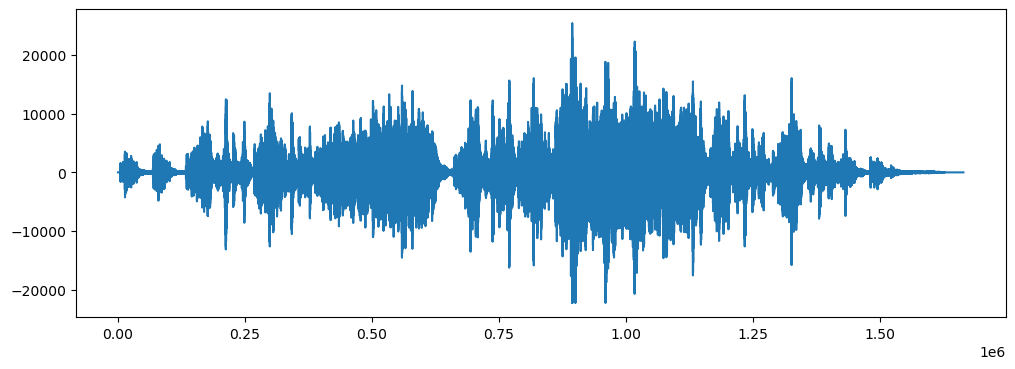
\includegraphics[width=\textwidth]{downSampled.png}
    \caption{Downsampled audio}
    \label{fig:downsampled audio}
\end{figure}

That being so, our focus will be narrowed to a specific region within the audio for enhanced visualization. This defined region will serve as our focal point for visualization throughout the project and it is represented by Figure \ref{fig:Observation Region}.

\begin{figure}[h]
    \centering
    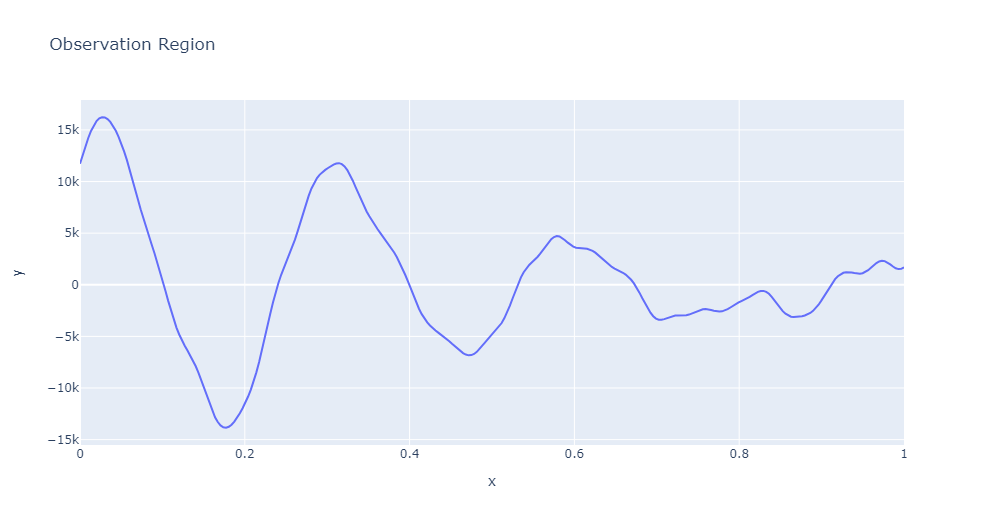
\includegraphics[width=\textwidth]{ObservationRegion.png}
    \caption{Observation Region}
    \label{fig:Observation Region}
\end{figure}
\newpage
\subsection{Down Sampling}

From the original audio, we generate a downsampled version intended for use as a low-bitrate audio suitable for interpolation and subsequent comparison.  \\

The downsampling process involves creating a new array, where each element corresponds to every $n$-th element in the original audio array. Let's denote the original audio matrix by $A_o$ with length $p$ and the downsampled audio as $A_n$ with length $q$, where $n$ is the downsampling factor.



$$ A_n[i] = A_o[n.i] \ , \   \ \  0 \leq i \leq {p \over n}$$
\noindent
The down-sampling function is implemented as follows:
\begin{lstlisting}[language=Python, caption={Down Sampling Function}]
def downsample_audio(original_audio, n):
    A_n = []
    new_sample_rate = original_audio[0] // n
    
    # Iterate through the original audio data and select every nth element
    for i in tqdm(range(len(original_audio[1]))):
        if i % n == 0:
            A_n.append(original_audio[1][i])
    
    return new_sample_rate, A_n
\end{lstlisting} 

Figure \ref{fig:orig_vs_downsampled} illustrates the disparity between the original audio signal and its downsampled counterpart by plotting the data points within the specified observation region. \\


\begin{figure}[h]
    \centering
    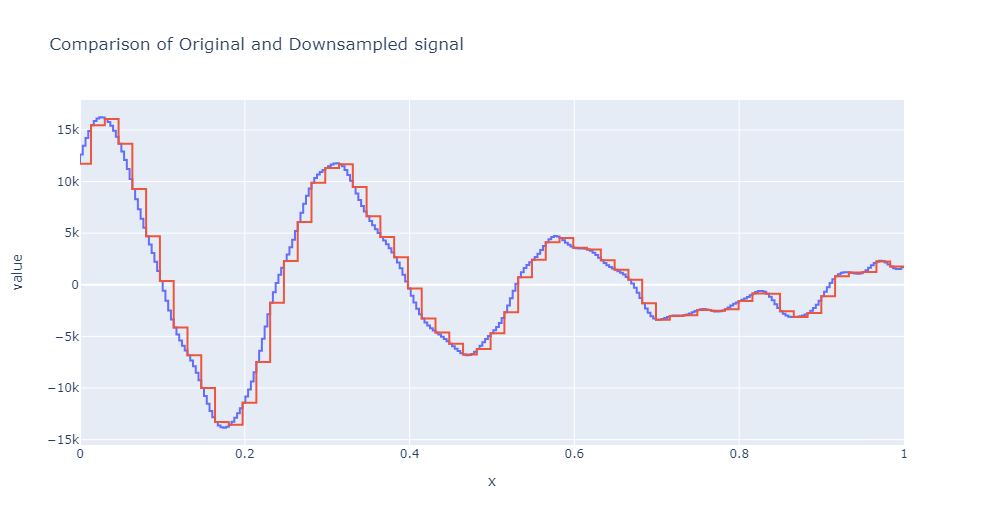
\includegraphics[width=\textwidth]{OrigVsDownSampled.png}
    \caption{Comparison of Original and Downsampled signal}
    \label{fig:orig_vs_downsampled}
\end{figure}

\newpage
\subsection{Linear Interpolation}

Linear Interpolation, a fundamental method for reconstructing downsampled audio to a higher sample rate, offers simplicity and effectiveness in bridging the gaps between data points. This technique aims to create a linear transition between consecutive observations, providing a straightforward yet valuable approach to upsampling.\\

The linear interpolation process commences with the creation of arrays \texttt{x\_observed} and \texttt{y\_observed}, representing the observed data points from the audio. Subsequently, a new set of x values (\texttt{x}) is generated based on the target sample rate. The \texttt{np.interp} function is then employed to perform the linear interpolation, filling in the gaps and producing the upsampled audio data.



\begin{lstlisting}[language=Python, caption={Linear Interpolation Function}]
def Linear_Interpolate(audio, target_sample_rate):
    x_observed = np.linspace(0.0, 1.0, len(audio[1]))
    y_observed = audio[1]
    x = np.linspace(min(x_observed), max(x_observed),
                    num=(len(audio[1]) * (target_sample_rate // audio[0])))
    y = np.interp(x, x_observed, y_observed)
    return target_sample_rate, y
\end{lstlisting} 
 
This function takes the original audio as input along with the target sample rate and performs linear interpolation to generate the upsampled audio.

\subsubsection{Results}

The application of Linear Interpolation is showcased in Figure \ref{fig:linear_interpolation}, providing a visual comparison of the original audio, the downsampled version, and the linearly interpolated audio. The root mean squared error calculation indicates that the upscaled audio differs from the original by 2.42\%.\cite{wiki_rmsd}

Despite its simplicity, linear interpolation proves to be a reliable method for upsampling, offering a balance between computational efficiency and preservation of audio integrity.

\begin{figure}[h]
    \centering
    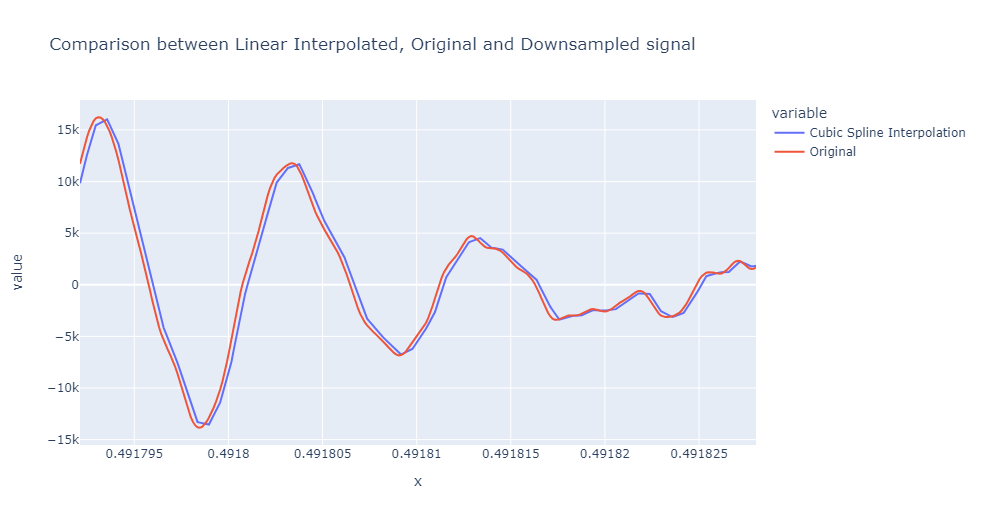
\includegraphics[width=\textwidth]{Linear.png}
    \caption{Comparison of Linear interpolated and Original signal}
    \label{fig:linear_interpolation}
\end{figure}



\newpage
\subsection{Piecewise cubic Hermite interpolating polynomial}
The Piecewise Cubic Hermite Interpolating Polynomial (Pchip) method is employed in this project for reconstructing the downsampled audio to a higher sample rate. Pchip interpolation is particularly useful in achieving smooth transitions between data points, ensuring a continuous and differentiable interpolation. \\

The Pchip interpolation process begins by creating arrays \texttt{x\_observed} and \texttt{y\_observed}, representing the observed data points from the audio. Subsequently, a new set of x values (\texttt{x}) is generated based on the target sample rate. The \texttt{pchip\_interpolate} function from the \texttt{scipy.interpolate} module is then applied to perform the interpolation and obtain the upsampled audio data.



\begin{lstlisting}[language=Python, caption={Piecewise cubic Hermite interpolating polynomial Function}]
from scipy.interpolate import pchip_interpolate

def Pchip_interpolate(audio,target_sample_rate):
    x_observed = np.linspace(0.0, 1.0, len(audio[1]))
    y_observed = audio[1]
    x = np.linspace(min(x_observed), max(x_observed), num=(len(audio[1])*(target_sample_rate//audio[0])))
    y = pchip_interpolate(x_observed, y_observed, x)
    return target_sample_rate,y
\end{lstlisting} 

\subsubsection{Results}

The application of Piecewise Cubic Hermite Interpolating Polynomial is visualized in Figure \ref{fig:pchip}, providing a comparative analysis of the original audio, the downsampled version, and the Pchip interpolated audio. The root mean squared error calculation indicates that the upscaled audio differs from the original by 2.418\%. \cite{wiki_rmsd}

The Pchip method excels in preserving the shape and smoothness of the original audio signal, making it a valuable technique for applications where maintaining the continuity of the signal is essential.

\begin{figure}[h]
    \centering
    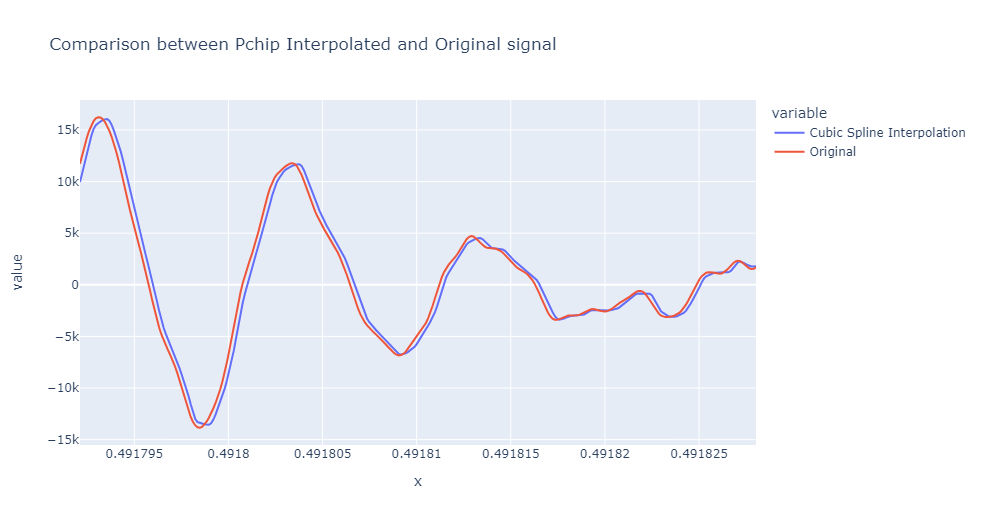
\includegraphics[width=\textwidth]{pchip.png}
    \caption{Comparison of Pchip Interpolated and Original signal}
    \label{fig:pchip}
\end{figure}

\newpage
\subsection{Cubic Spline Interpolation}

Cubic Spline Interpolation, a method employed in reconstructing downsampled audio to a higher sample rate, leverages the flexibility of cubic polynomials to ensure a smooth and continuous interpolation. The implementation involves the utilization of the \texttt{CubicSpline} function from the \texttt{scipy.interpolate} module.


\begin{lstlisting}[language=Python, caption={Cubic Spline Interpolation}]
from scipy.interpolate import CubicSpline

def CubicSpline_interpolate(audio, target_sample_rate):
    x = np.linspace(0,1,len(audio[1]))
    y = audio[1]
    cs = CubicSpline(x, y)
    xs = np.linspace(0, 1, (len(audio[1])*(target_sample_rate//audio[0])))
    return target_sample_rate, cs(xs)
\end{lstlisting} 

\subsubsection{Results}

The effectiveness of Cubic Spline Interpolation is illustrated in Figure \ref{fig:cubic_spline}, highlighting the comparison between the original audio, the downsampled version, and the Cubic Spline interpolated audio. The root mean squared error calculation indicates that the upscaled audio differs from the original by 2.418\%.\cite{wiki_rmsd} \\

The smoothness achieved by Cubic Spline Interpolation contributes to its ability to reconstruct the downsampled audio, making it a viable method for applications where preserving the continuity of the signal is crucial.

\begin{figure}[h]
    \centering
    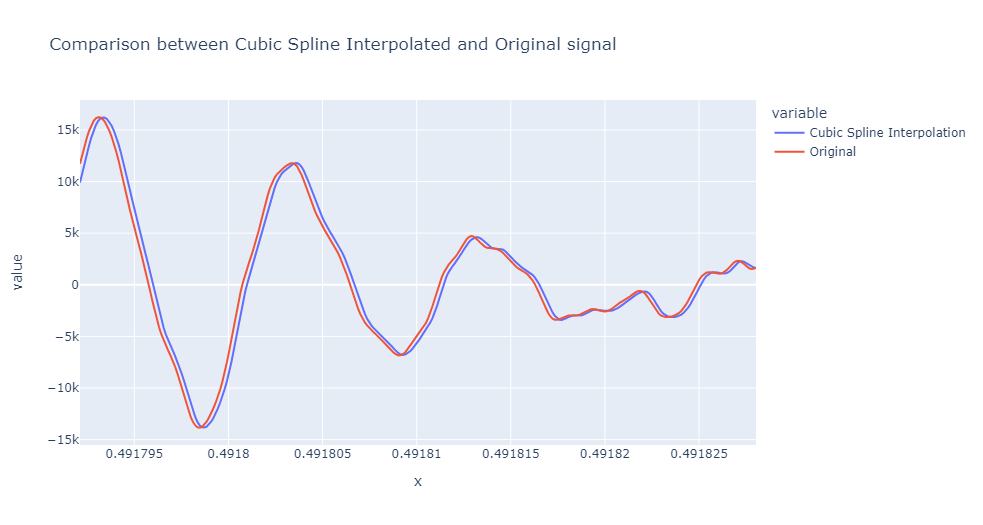
\includegraphics[width=\textwidth]{cubic_spline.png}
    \caption{Comparison of Cubic Spline Interpolated and Original signal}
    \label{fig:cubic_spline}
\end{figure}


\newpage

\section{Conclusion}

In the pursuit of enhancing audio quality through upsampling methods, this project investigated various interpolation techniques applied to a downsampled audio signal. The selected interpolation methods—Linear Interpolation, Piecewise Cubic Hermite Interpolating Polynomial (Pchip), and Cubic Spline Interpolation—were evaluated based on their ability to reconstruct the downsampled audio close to the original. \\

The visual comparisons and quantitative analysis revealed that linear interpolation exhibited the least error, resulting in a more faithful reconstruction of the downsampled audio compared to the original signal. This observation aligns with the goal of minimizing distortion and preserving the integrity of the audio waveform.


\begin{figure}[h]
    \centering
    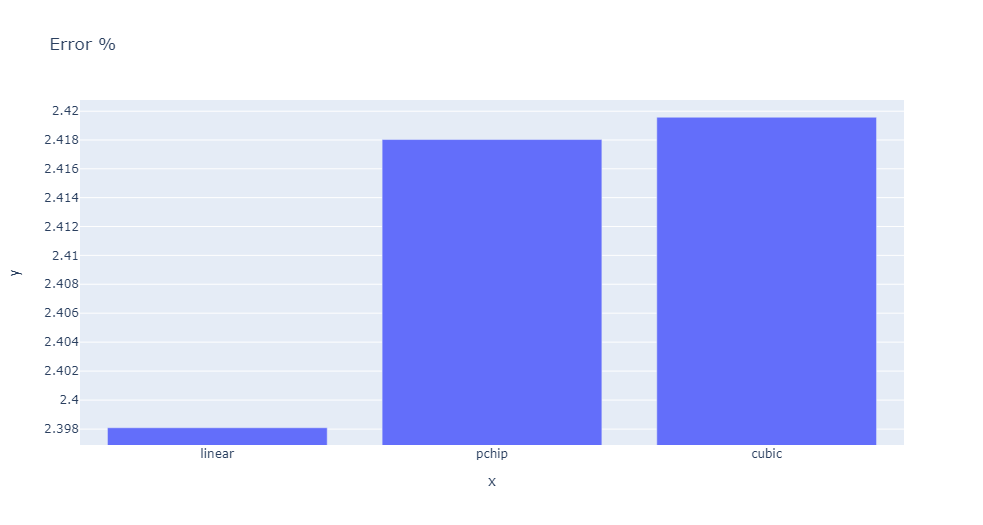
\includegraphics[width=\textwidth]{conclusion.png}
    \caption{Errors in different methods}
    \label{fig:conclusion}
\end{figure}


While the choice of interpolation method depends on specific use cases and desired outcomes, the findings of this study underscore the effectiveness of linear interpolation in achieving accurate audio upsampling. Further exploration into the interplay of different factors, such as downsampling ratios and signal characteristics, could provide valuable insights for refining audio upsampling techniques in future applications.

\newpage
\printbibliography[title={References}]

\end{document}
